
\chapter{Advanced Financial Models}

The Black--Scholes framework rests on two statistical pillars: log-returns are Gaussian, and volatility is constant.
Chapter~5 already hinted, through the volatility smile, that the market itself does not believe either.
In this chapter we confront the model with the data and repair it in two directions.
First, we introduce the \emph{stable distributions} of L\'evy, whose fat tails describe the empirical statistics of returns far better than the Gaussian; second, we promote the volatility to a stochastic process of its own, obtaining the \emph{stochastic volatility} models --- Stein--Stein, Heston, and their relatives --- that are the workhorses of modern quantitative finance.
The chapter closes by redoing Black--Scholes in the Heston world, where a new and instructive obstacle appears: volatility cannot be hedged with the stock alone.
% CLAUDE NOTE (unreviewed PDF): These notes are unreviewed but "mostly good."
% Original reasoning is preserved; expansions and corrections are noted in comments.

Before any statistics, Figure~\ref{fig:sp500-vs-gbm} explains both why the GBM conquered finance and why this chapter is necessary.
The upper panel shows ten years of the real S\&P\,500; the lower panel shows a geometric Brownian motion simulated with the \emph{same} drift and the \emph{same} volatility, estimated from those very data.
At a glance the two are remarkably alike --- same trend, same jitter, same look at every scale --- which is precisely the mimicry that made the GBM the default model of Chapter~5.
Look longer, though, and the real series gives itself away: the cliff of February--March 2020, when the index lost a third of its value in four weeks with single days beyond $-12\%$, has no counterpart in the simulated panel --- and never will, because in a Gaussian world a $12\sigma$ day is not rare but essentially impossible.
Everything that follows in this chapter is, in one way or another, the statistics of that difference.

% Real-data figure; generated by images/code_for_images/sp500_returns.py from FRED series SP500.
\begin{figure}[h!]
\centering
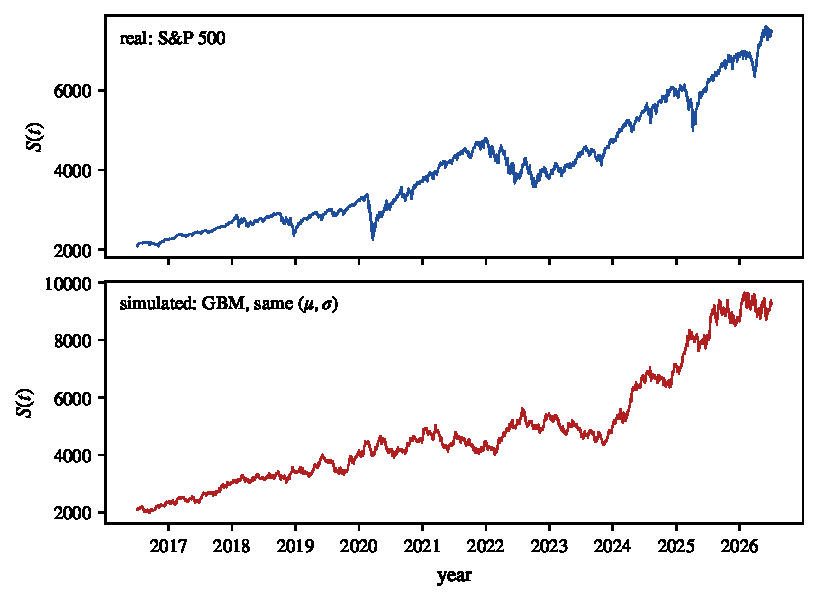
\includegraphics[width=0.88\textwidth]{images/sp500_vs_gbm.pdf}
\caption{Top: the S\&P\,500, daily closes 2016--2026 (FRED series SP500). Bottom: a geometric Brownian motion simulated with the same starting value and the same daily drift and volatility estimated from the data. The two are nearly indistinguishable by eye --- except for the 2020 crash in the real series, whose violence the Gaussian model cannot produce. Generated by \texttt{images/code\_for\_images/sp500\_returns.py}.}
\label{fig:sp500-vs-gbm}
\end{figure}


\section{Empirical properties of log-returns}

Let us first recall what the GBM predicts, so that we know exactly what to test.
For $dS = \mu S\,dt + \sigma S\,dW_t$, the log-returns satisfy
\begin{equation}
\mathbb{E}\!\biggl[\ln\frac{S(t+\Delta t)}{S(t)}\biggr] = \mu^*\Delta t, \qquad \mu^* = \mu - \frac{\sigma^2}{2},
\qquad
\mathrm{Var}\!\biggl[\ln\frac{S(t+\Delta t)}{S(t)}\biggr] = \sigma^2\Delta t,
\end{equation}
and shifting the time window, $t\to t+\tau$, $t+\Delta t\to t+\Delta t+\tau$, changes nothing: the returns are stationary, consistent with $\delta t = t_j - t_i = (t_j + \Delta t) - t_j$.
For the price itself the model gives
\begin{equation}
\mathbb{E}[S(t)] = S_0\, e^{\mu t}, \qquad \mathrm{Var}[S(t)] = S_0^2\, e^{2\mu t}\bigl(e^{\sigma^2 t}-1\bigr),
\end{equation}
although in reality $\mu$ itself changes over the years --- a first warning sign.

The decisive test is the histogram.
Take a real time series, compute the log-returns, extract the empirical mean and standard deviation $\mu_e \leftrightarrow m$, $\sigma_e \leftrightarrow s$, and superimpose on the histogram the Gaussian that the model predicts,
\begin{equation}
\mathrm{PDF}\!\bigl\{\ln r_{\Delta t}(t)\bigr\} \approx \mathcal{N}(\mu_e, \sigma_e) = \frac{1}{\sqrt{2\pi\sigma_e^2}}\,\exp\!\biggl\{-\frac{(\ln r_{\Delta t}(t) - \mu_e)^2}{2\sigma_e^2}\biggr\}.
\end{equation}
The fit fails, and it fails in a characteristic way, shown on real data in Figure~\ref{fig:sp500-hist}: the empirical distribution is far more peaked at the centre and, above all, far heavier in the tails.
Extreme returns --- crashes and rallies --- occur orders of magnitude more often than any Gaussian allows.
The returns are \emph{not} normally distributed, and we need a family of distributions built to accommodate this.

% Figure after the course slides; generated by images/code_for_images/sp500_stylized.py
\begin{figure}[h!]
\centering
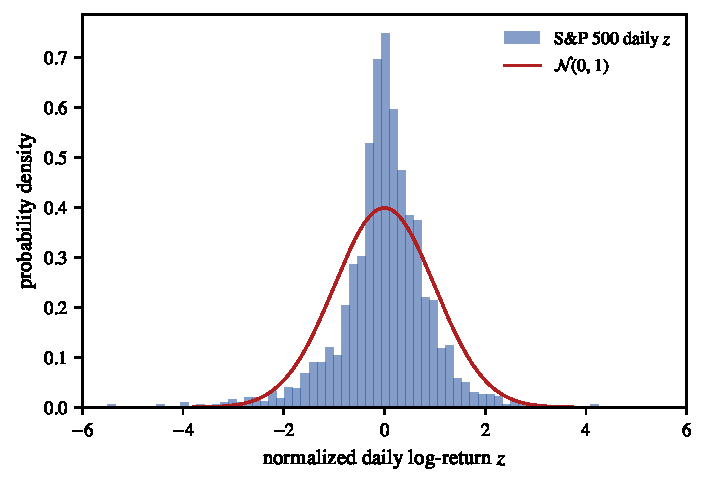
\includegraphics[width=0.72\textwidth]{images/sp500_hist.pdf}
\caption{The histogram test on real data: normalized daily log-returns of the S\&P\,500 (2016--2026, FRED series SP500) against the Gaussian with the same mean and variance. The empirical distribution has a sharper central body and far heavier tails --- returns beyond $\pm4\sigma$, essentially impossible for the Gaussian, are clearly populated. Generated by \texttt{images/code\_for\_images/sp500\_stylized.py}.}
\label{fig:sp500-hist}
\end{figure}


\section{Stable distributions}\label{sec:stable-distributions}

The appropriate family was identified by L\'evy, and imported into finance by Mandelbrot: the \emph{stable distributions}, whose theory is also known as the \emph{generalized Central Limit Theorem} (generalized CLT), with contributions by Gnedenko.
Why ``generalized''?
The ordinary CLT says that sums of i.i.d.\ variables with \emph{finite variance} converge to the Gaussian; the generalized version asks the bolder question --- what are \emph{all} the possible limits of such sums, finite variance or not? --- and the answer is precisely the stable family.

A stable distribution is characterized by four interlocking properties, which we examine in turn: stability under convolution, a closed-form characteristic function, power-law asymptotic behaviour, and the corresponding cumulative distribution function (CDF).

\subsection{Stability}

Let $X_1, X_2$ be i.i.d.\ random variables with PDF $P(x)$, so that $P_2(x_1, x_2) = P(x_1)P(x_2)$, and consider their sum $S_2 = X_1 + X_2$ (so that $X_2 = S_2 - X_1$).
The PDF of the sum is the convolution
\begin{equation}
P_2(S_2) = \int dx\, P(x)\, P(S_2 - x) = P * P.
\end{equation}
Convolutions are unwieldy; Fourier transforms turn them into products.
Defining the \emph{characteristic function} $\tilde\phi(k)=\mathcal{F}[P]$,
\begin{equation}
\mathcal{F}\bigl[P_2(S_2)\bigr] = \tilde\phi_2(k) = \int dx\, e^{ikx}\, P_2(S_2) = \mathcal{F}[P*P] = \mathcal{F}[P]\cdot\mathcal{F}[P] = \tilde\phi^2(k),
\end{equation}
and for $N$ i.i.d.\ variables $X_1,\ldots,X_N$ with $S_N = \sum_{i=1}^{N} X_i$,
\begin{equation}
\mathcal{F}[P_2(S_N)] = \tilde\phi^N(k),
\end{equation}
generically a leptokurtic (heavy-tailed relative to its width) distribution.
A distribution is called \emph{stable} when this operation does not change its shape: the sum has the same distribution as the summands, up to a rescaling.

The Gaussian is the prototype.
For $P_0(x) = \frac{1}{\sqrt{2\pi}\sigma}\, e^{-x^2/(2\sigma^2)}$, with scale parameter $\sigma$, the characteristic function is
\begin{equation}
\tilde\Phi(k) = \int dx\, e^{ikx}\, P_0(x) = \exp\!\Bigl\{-\frac{\sigma^2 k^2}{2}\Bigr\},
\end{equation}
so that
\begin{equation}
\tilde\phi_2(k) = \mathcal{F}[P*P] = e^{-\sigma^2 k^2} \quad\Longrightarrow\quad \mathcal{F}^{-1}[\tilde\phi_2(k)] = P_0(x, N=2):
\end{equation}
the sum of two Gaussians is again a Gaussian --- the Gaussian is stable.
How does the scale grow?
Rewriting the $N=2$ result,
\begin{equation}
P_0(x, N=2) = \frac{1}{\sqrt{2\pi(2\sigma^2)}}\, \exp\!\biggl\{-\frac{x^2}{2\cdot 2\sigma^2}\biggr\} = \frac{1}{\sqrt{2}}\,\frac{1}{\sigma_2}\, P_0\!\Bigl(\frac{x}{\sigma_2}\Bigr),
\end{equation}
and in general
\begin{equation}
P_N(x, N) = \frac{1}{a_N}\, P_0\!\Bigl(\frac{x}{a_N}\Bigr), \qquad a_N = \sqrt{N}\, \sigma = N^{1/\alpha}\sigma, \quad \alpha = 2,
\end{equation}
where the $a_N$ are rescaling factors.
The exponent $\alpha$ appearing in $a_N = N^{1/\alpha}$ is the \emph{characteristic exponent} (or \emph{L\'evy index}) of the distribution; for the Gaussian, $\alpha=2$, which is just the familiar $\sqrt{N}$ growth of a random walk.
As we now see, other values of $\alpha$ are possible --- and each governs a different, self-consistent statistical world.

\subsection{The Cauchy distribution}

The most instructive non-Gaussian member of the family is the \emph{Cauchy} distribution (the Lorentzian of spectroscopy), which realizes $\alpha=1$:
\begin{equation}
P_c(x) = \frac{\delta}{\pi}\,\frac{1}{\delta^2 + x^2}, \qquad \delta = \text{scale parameter}.
\end{equation}
Its characteristic function is the two-sided exponential
\begin{equation}
\tilde\phi(k) = \mathcal{F}[P_c(x)] = e^{-\delta|k|},
\end{equation}
and stability is verified at sight:
\begin{equation}
\tilde\phi_2(k) = e^{-2\delta|k|} \quad\Longrightarrow\quad P_c(x, N=2) = \frac{2\delta}{\pi}\,\frac{1}{4\delta^2+x^2} = \frac{1}{a_2}\,P_c\!\Bigl(\frac{x}{a_2}\Bigr),
\end{equation}
a Cauchy again, with rescaling $a_N = N^{1/\alpha}$, $\alpha=1$: the scale of the sum grows \emph{linearly} in $N$, much faster than the Gaussian $\sqrt{N}$.
Asymptotically $P_c(x) \sim 1/x^{1+\alpha} = 1/x^{2}$ for $|x|\to\infty$, and this slow power-law decay has a startling consequence: the Cauchy distribution has \emph{no finite mean and no finite variance}.
It is a pathological but deeply instructive object --- a perfectly legitimate, normalizable distribution for which the standard toolkit of means and variances simply does not apply.
The family of stable laws interpolates between these behaviours, guided by the index $\alpha$.

\subsection{General $\alpha$-stable distributions}

For a general symmetric $\alpha$-stable distribution the characteristic function is
\begin{equation}
\tilde\phi_\alpha(k) = \exp\!\bigl\{-\delta|k|^\alpha\bigr\}, \qquad \forall\, \alpha \text{ admissible and } \delta \text{ (scale)},
\end{equation}
a \emph{stretched exponential} in $k$ for $\alpha\in(0,2)$.
The two cases already met are recovered as $\delta = \frac{\sigma^2}{2}$, $\alpha=2$ (Gaussian) and $\delta > 0$, $\alpha=1$ (Cauchy).
The admissible range is $0 < \alpha \le 2$, and within it the moments deteriorate progressively: for $1 < \alpha < 2$ the variance does not exist; for $0 < \alpha \le 1$ even the mean is gone.
Such distributions have no characteristic scale --- they are \emph{scale-free}.
The density itself is recovered by inverse Fourier transform,
\begin{equation}
P_\alpha(x) = \frac{1}{2\pi}\int dk\, e^{-ikx}\, e^{-\delta|k|^\alpha}, \qquad \int dx\, P_\alpha(x) = 1,
\end{equation}
which has closed form only in special cases ($\alpha=2$, $\alpha=1$), but whose properties are known in general.

\subsection{Asymptotic behaviour and CDF}

The third property is the one that matters most for data analysis: for every $\alpha<2$, the tails of the density decay as a \emph{power law},
\begin{equation}
P_\alpha(x) \propto \frac{C_\alpha}{|x|^{1+\alpha}}, \qquad |x|\to\infty.
\end{equation}
In practice one works with the fourth property, the cumulative distribution,
\begin{equation}
P_<(x) = \int_{-\infty}^{x}\! P(x')\, dx', \qquad P_>(x) = \int_x^{+\infty}\! P(x')\, dx' = 1 - P_<(x),
\end{equation}
because integrating the histogram tames the statistical noise in the tail.
Writing $\alpha' = \alpha + 1$ for the density exponent (so that $0 < \alpha' \le 3$ delimits the L\'evy regime), the tail of the CDF follows by direct integration:
\begin{equation}
P_>^*(x) = \int_x^{+\infty}\!dx'\; P_\alpha(x') \;\xrightarrow{|x|\to\infty}\; C_\alpha\int_x^{\infty}\!dx'\; x'^{-\alpha'} = \frac{C_\alpha}{\alpha'-1}\,x^{-(\alpha'-1)} = \frac{C_\alpha}{\alpha}\,x^{-\alpha}.
\end{equation}
Taking logarithms of both sides,
\begin{equation}
\ln P_>^*(x) = \ln\frac{C_\alpha}{\alpha} - \alpha\ln x,
\end{equation}
so in a \emph{log-log plot} the tail is a straight line of slope $-\alpha$: this is the standard experimental signature, and the standard way of measuring $\alpha$ from data (Figure~\ref{fig:loglog-tail}).
The contrast with the Gaussian could not be sharper: $\ln P_0(x) \sim -x^2$ plunges quadratically, while $\ln P_\alpha(x) \sim -\alpha\ln x$ descends along a gentle straight line --- the fat tail.

\begin{figure}[h!]
\centering
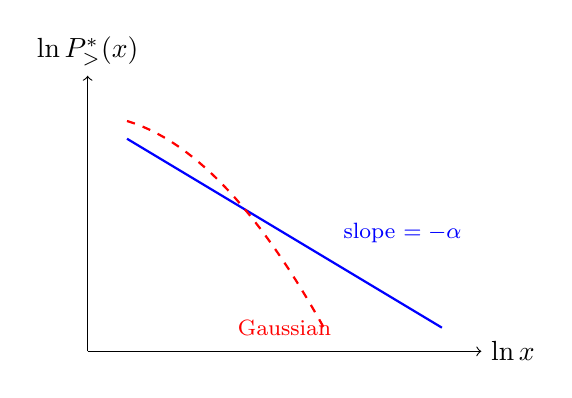
\begin{tikzpicture}
    \draw[->] (0,0) -- (5,0) node[right] {$\ln x$};
    \draw[->] (0,0) -- (0,3.5) node[above] {$\ln P_>^*(x)$};
    \draw[thick, blue, domain=0.5:4.5, samples=50] plot (\x, {3.0 - 0.6*\x});
    \node[blue, font=\footnotesize] at (4, 1.5) {slope $= -\alpha$};
    \draw[thick, red, dashed, domain=0.5:3, samples=50] plot (\x, {3.0 - 0.3*\x*\x});
    \node[red, font=\footnotesize] at (2.5, 0.3) {Gaussian};
\end{tikzpicture}
\caption{Tail of the cumulative distribution in a log-log plot: a stable law gives a straight line of slope $-\alpha$, while the Gaussian bends down quadratically. The straight-line tail is the experimental fingerprint of fat tails.}
\label{fig:loglog-tail}
\end{figure}

\subsection{Empirical evidence}

How do real markets score on this test?
The first measurement is due to Mandelbrot, who studied the daily log-returns of cotton prices and found a beautiful power-law tail with $\alpha \approx 1.7$; Fama repeated the analysis on stock returns with similar results (empirical analyses of asset prices for which Fama would receive the 2013 Nobel Prize in Economics).
% CLAUDE NOTE: the Fama Nobel mention is from the course slides, added 2026-07-06.
% CLAUDE NOTE: the notes attribute the stock-returns study to "Gnedenko (Fama)"; the standard
% reference for daily stock returns is Fama's 1965 study, while Gnedenko's contribution is the
% generalized CLT theory itself.
But a value $\alpha = 1.7 < 2$ is not acceptable at face value: it implies \emph{infinite variance}, hence in particular an undefined volatility --- awkward, for the quantity on which all of Chapter~5 was built.

The modern reference measurement is that of Mantegna and Stanley \cite{MantegnaStanley1995}, who analysed the S\&P\,500 at $\Delta t = 1$ minute over 1984--1989, using the standardized variable
\begin{equation}
z = \frac{\frac{\Delta S_{\text{SP}}(t)}{S(t)} - \mu}{\sigma},
\end{equation}
and found, once again, a stable-law behaviour with $\alpha \approx 1.4$.

The test is easy to repeat on modern data, and Figure~\ref{fig:sp500-ccdf} does so on ten years of daily S\&P\,500 closes.
The result is textbook material in the most literal sense: the empirical CCDF of the normalized returns tracks the Gaussian up to about two standard deviations and then departs from it spectacularly, following a straight power-law line of slope $\approx-3$ across the tail --- daily moves of $5\sigma$, which the Gaussian declares essentially impossible ($P_>\sim10^{-7}$), occur at the rate of a few per decade.
A CCDF slope of $-3$ corresponds to a density decaying as $|z|^{-4}$: this is precisely the \emph{inverse quartic law} that we are about to meet in the next subsection, and it lies \emph{outside} the L\'evy range $\alpha<2$ --- a first hint that the pure stable law cannot be the whole story.

% Real-data figure; generated by images/code_for_images/sp500_returns.py from FRED series SP500.
\begin{figure}[h!]
\centering
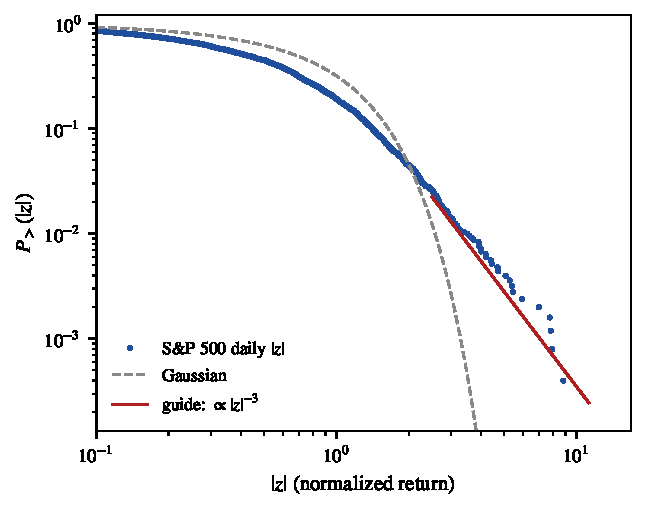
\includegraphics[width=0.62\textwidth]{images/sp500_ccdf.pdf}
\caption{Complementary CDF of the absolute normalized daily log-returns $|z|$ of the S\&P\,500 (2016--2026, FRED series SP500), in log-log scale, against the Gaussian prediction (dashed) and the inverse-cubic guide line $\propto|z|^{-3}$ (red). The fat tail --- the straight-line regime --- is the empirical refutation of the GBM hypothesis. Generated by \texttt{images/code\_for\_images/sp500\_returns.py}.}
\label{fig:sp500-ccdf}
\end{figure}
Two observations enrich the picture.
First, the S\&P\,500 aggregates $500$ assets, and its distribution is non-Gaussian because the components are \emph{not independent} --- when they fall, they fall together, so the standard CLT does not apply to the aggregation; disentangling such cross-correlations requires \emph{random matrix theory}.
Second, the scaling is impressive: the same law, with the same $\alpha$, holds across different time horizons $\Delta t$, with the PDF collapsing as $\mathrm{PDF}\{r(\Delta t)\} \sim \Gamma^*(\Delta t)$ and the CDF as $r^*(\Delta t)$ --- the self-similarity of stable laws at work in real data.

\subsection{Truncated stable distributions}

The resolution of the infinite-variance puzzle is that the true tail is \emph{not} a pure stable law all the way to infinity.
The far tail is better modelled by a power law \emph{truncated by an exponential},
\begin{equation}
P_{\alpha,\lambda}(x) \sim |x|^{-(1+\alpha)}\, e^{-\lambda|x|},
\end{equation}
% CLAUDE NOTE (unreviewed): the notes' exponent reads "(α−1)" with a positive sign, which
% would not be normalizable; the truncated Lévy distribution keeps the tail exponent −(1+α)
% of the pure stable law, multiplied by the exponential cutoff.
which preserves the stable behaviour over the observable range while restoring a finite variance.
An equally popular parametrization is the \emph{Student-$t$} distribution,
\begin{equation}
P_S(t) = C_S\biggl(1 + \frac{x^2}{v\hat\sigma^2}\biggr)^{-\frac{v+1}{2}},
\end{equation}
where $\hat\sigma$ is a scale parameter and $v$ a shape parameter (the number of degrees of freedom).
For $v=3$ the asymptotic tail decays as $x^{-4}$ --- the \emph{inverse quartic law} --- which is compatible with a large body of empirical observations.\footnote{The Student-$t$ arises naturally as a mixture of Gaussians whose variance is itself random ($\chi^2$-distributed) --- a first hint that random volatility and fat tails are two faces of the same phenomenon. This is the parametric approach to fitting the PDF of returns.}


\section{Volatility}\label{sec:adv-volatility}

The second pillar to re-examine is the volatility.
In reality $\sigma$ is not constant --- and worse, it is a \emph{hidden} quantity: no market quotes it directly, and extracting it is a delicate statistical task.
Throughout this section the basic observable is the log-return
\begin{equation}
dX_t = \ln\frac{S(t+\Delta t)}{S(t)} - S(t).
\end{equation}
% CLAUDE NOTE: The notes define dX as the log-return; the subtraction of S(t) is likely
% shorthand for the centered return (subtracting the mean μ*Δt).

Three estimators of volatility are in common use, in increasing order of temporal resolution.

The first is the \emph{historical volatility}, extracted from the sample variance of the time series, exactly as described in Chapter~5 (Section~\ref{sec:volatility}).

The second is the \emph{high-frequency volatility}, built from the mean absolute return rather than the squared one,
\begin{equation}
\sigma_{\text{hf}} = \frac{1}{N-1}\sum_{i=1}^{N}|dX_i|,
\end{equation}
with $\alpha$ the exponent of the associated $P(x)$.
To relate it to $\sigma$, assume for a moment Gaussian returns, $P(x)=\mathcal{N}(0,\sigma^2)$; then
\begin{equation}\begin{split}
\sigma_{\text{hf}} = \mathbb{E}[|x|] &= \int dx\,|x|\,P(x) = 2\int_0^{\infty}\!dx\; x\, P(x)\\
&= \frac{2}{\sqrt{2\pi}\,\sigma}\int_0^{\infty}\!dx\; x\, e^{-x^2/(2\sigma^2)}
= \sqrt{\frac{2}{\pi}}\,\sigma \approx 0.8\,\sigma,
\end{split}\end{equation}
so the mean absolute return is a proxy that \emph{under}estimates $\sigma$ by a known factor $\sqrt{2/\pi}$ --- easily corrected, and statistically more robust against outliers than the sample variance.

The third and most direct is the \emph{instantaneous volatility}, read off the SDE itself.
From
\begin{equation}
\ln\frac{S(t+\Delta t)}{S(t)} = \mu^*\Delta t + \sigma\,\Delta W_t,
\end{equation}
the square of the return is dominated, for small $\Delta t$, by the noise term ($\Delta W^2\sim\Delta t$, while the drift contributes only at order $\Delta t^2$), so that
\begin{equation}
\biggl(\ln\frac{S(t+\Delta t)}{S(t)}\biggr)^{\!2} \;\xrightarrow{\ \Delta t\to0\ }\; \sigma^2\Delta t
\quad\Longrightarrow\quad
\sigma_{\text{ist}} = \sqrt{\frac{|dX_t|^2}{\Delta t}} = \frac{|dX_t|}{\sqrt{\Delta t}},
\end{equation}
a volatility measured return by return --- as local as the data allow.


\section{Volatility clustering}\label{sec:vol-clustering}

With an instantaneous estimator in hand, one can finally look at volatility \emph{as a time series} --- and what one sees is striking.
Volatility is \emph{intermittent}: long quiet stretches alternate with sudden bursts of turbulence, in a pattern strongly reminiscent of the velocity field of a turbulent fluid.
Figure~\ref{fig:sp500-clustering} shows the phenomenon on real data --- ten years of daily S\&P\,500 log-returns: the calm of 2017 and the fury of March 2020 are not different draws from one distribution, they are different \emph{regimes}, and large moves visibly arrive in clusters.
The statistics makes the analogy quantitative.

% Real-data figure; generated by images/code_for_images/sp500_returns.py from FRED series SP500.
\begin{figure}[h!]
\centering
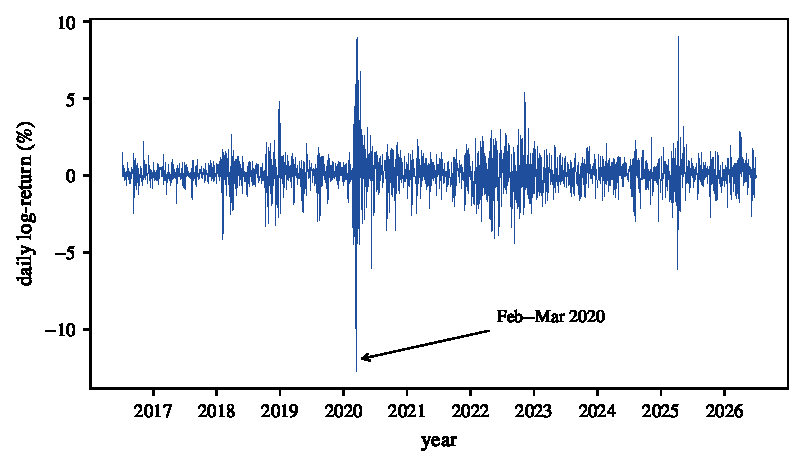
\includegraphics[width=0.9\textwidth]{images/sp500_logreturns.pdf}
\caption{Daily log-returns of the S\&P\,500, 2016--2026 (FRED series SP500). Quiet stretches alternate with bursts of turbulence --- most dramatically the COVID crash of February--March 2020 --- and large returns of either sign cluster together: this is volatility clustering, incompatible with a constant $\sigma$. Generated by \texttt{images/code\_for\_images/sp500\_returns.py}.}
\label{fig:sp500-clustering}
\end{figure}
The log-returns themselves are essentially uncorrelated,
\begin{equation}
\mathbb{E}[dX_i \cdot dX_{i+\tau}] \approx 0 \quad (\text{decaying within minutes}),
\end{equation}
as the EMH demands --- if returns were predictable, they would be arbitraged away.
But their \emph{absolute values} are strongly and persistently correlated, with a slow power-law decay of the autocorrelation,
\begin{equation}
\mathbb{E}\bigl[|dX_i| \cdot |dX_{i+\tau}|\bigr] \sim \tau^{-\beta}, \qquad \beta \approx 0.3,
\end{equation}
% CLAUDE NOTE: the notes (PDF 6, page 5) write "~ τ^β, β ≈ 0.8"; an autocorrelation that
% DECAYS requires a negative exponent, and the measured value for |returns| of the S&P 500
% is β ≈ 0.3 (Gopikrishnan et al. 1999, as in the course slides). Corrected at the
% author's request (2026-07-06).
so a large move today makes large moves likely for days and weeks to come, in either direction\cite{Gopikrishnan1999}.
Figure~\ref{fig:sp500-acf} shows both facts at once on our daily data: the autocorrelation of the returns collapses into the statistical noise band within a lag or two, while that of the absolute returns stays positive for months, decaying along the $\tau^{-0.3}$ line.

% Figure after the course slides; generated by images/code_for_images/sp500_stylized.py
\begin{figure}[h!]
\centering
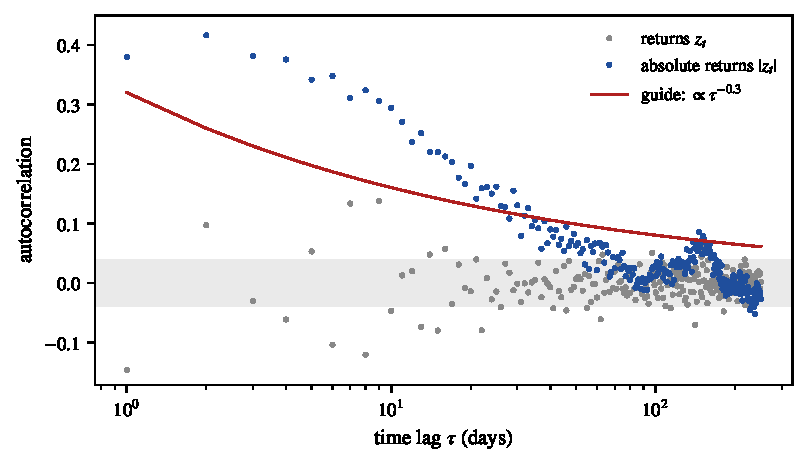
\includegraphics[width=0.85\textwidth]{images/sp500_acf.pdf}
\caption{Sample autocorrelation of the daily S\&P\,500 log-returns (grey) and of their absolute values (blue), against the time lag $\tau$; the shaded band is the $95\%$ noise level. Returns are uncorrelated beyond a day --- efficient-market behaviour --- while their magnitudes remain correlated for months, with the power-law decay $\propto\tau^{-0.3}$ (red): returns are uncorrelated but not independent. Generated by \texttt{images/code\_for\_images/sp500\_stylized.py}.}
\label{fig:sp500-acf}
\end{figure}
The two facts together imply that
\begin{equation}
\sigma_{\text{hf}}^2 \neq \sigma_{\text{ist}}^2,
\end{equation}
i.e.\ the log-returns, though uncorrelated, are \emph{not independent} --- the dependence hides in their magnitudes.
This is \emph{volatility clustering}, and it kills the constant-$\sigma$ hypothesis for good; even the distribution of the volatility itself turns out to have heavy tails, and is well fitted empirically by a log-normal or an inverse-Gamma law\cite{BouchaudPotters2003}.
% CLAUDE NOTE: the log-normal / inverse-Gamma fits are from the course slides
% (after Bouchaud & Potters), added 2026-07-06.
The natural response is to give $\sigma$ its own dynamics.


\section[Fractional Brownian motion*]{Fractional Brownian motion\texorpdfstring{$^*$}{*}}\label{sec:fbm}
% ============================================================================
% SECTION WRITTEN FROM SCRATCH (asterisk convention): "moto browniano frazionario"
% is listed in the official course program ("slides and other/programma.pdf",
% section "Dinamica dei Mercati Finanziari") but does not appear in the handwritten
% notes; only a passing mention of fractional models survives in the slides.
% Written 2026-07-06 from Mandelbrot & Van Ness (1968) and Gatheral et al. (2018).
% ============================================================================

Before turning correlated volatility into a model, it is worth meeting the stochastic process invented precisely to carry \emph{long-range memory}: the \emph{fractional Brownian motion} (fBM) of Mandelbrot and Van~Ness\cite{MandelbrotVanNess1968}.
The Wiener process of Chapter~3 has independent increments by construction; fBM relaxes exactly this axiom, and nothing else.
It is the Gaussian process $B_H(t)$ with $B_H(0)=0$, zero mean, and covariance
\begin{equation}
\langle B_H(t)\, B_H(s)\rangle = \frac{1}{2}\bigl(t^{2H} + s^{2H} - |t-s|^{2H}\bigr),
\end{equation}
where the parameter $H\in(0,1)$ is called the \emph{Hurst exponent}.
For $H=\tfrac12$ the covariance collapses to $\min(t,s)$, and one recognizes the autocorrelation of the ordinary Wiener process: fBM is a one-parameter deformation of Brownian motion, with $H$ dialling the memory.

Three properties follow directly from the covariance.
First, the variance grows \emph{anomalously},
\begin{equation}
\mathrm{Var}[B_H(t)] = t^{2H},
\end{equation}
faster than linearly for $H>\tfrac12$ (superdiffusion) and slower for $H<\tfrac12$ (subdiffusion) --- the process is self-similar with exponent $H$, generalizing the $\sqrt{t}$ scaling of Chapter~2.
Second, the increments are stationary but \emph{correlated}: a short computation with the covariance shows that the correlation of two successive unit increments equals $2^{2H-1}-1$, which is positive for $H>\tfrac12$ (\emph{persistence}: a rise tends to be followed by a rise), negative for $H<\tfrac12$ (\emph{antipersistence}: a rise tends to be followed by a fall), and zero only at $H=\tfrac12$.
Third --- and this is the price of memory --- for $H\neq\tfrac12$ the process is \emph{neither Markov nor a semimartingale}: the entire framework of Chapters~3 and~4, from Chapman--Kolmogorov to the It\^o integral, does not apply to it as it stands.
Long-range dependence is bought at the cost of the whole toolbox.

Why pay that price?
Because the volatility, as we have just measured, \emph{has} long-range memory: the power-law decay of Figure~\ref{fig:sp500-acf} is precisely the kind of correlation that no Markov process can sustain and that fBM carries natively.
The modern \emph{rough volatility} programme models the log-volatility as a fractional Brownian motion, and the empirical estimates are striking: fitting high-frequency data gives a very small Hurst exponent, $H\approx0.1$ --- volatility is not only stochastic but \emph{rough}, far more irregular than a Brownian path --- while reproducing the smile and the clustering with remarkably few parameters\cite{GatheralEtAl2018}.
For the underlying price itself, on the other hand, $H\ne\tfrac12$ would imply predictable returns and hence arbitrage, so the EMH pins the price's Hurst exponent to $\tfrac12$; the memory lives in the volatility, not in the direction of the moves --- in exact agreement with the two panels of Figure~\ref{fig:sp500-acf}.


\section{Stochastic volatility models}\label{sec:stoch-vol}

To model a time-varying $\sigma$, one couples the price to a second stochastic process $Y(t)$ that drives the volatility.
The general \emph{stochastic volatility} model is the two-dimensional SDE system
\begin{align}
(1)\quad & dS(t) = \mu\, S(t)\, dt + f[Y(t)]\, S(t)\, dW_1(t), \label{eq:sv-stock} \\[4pt]
(2)\quad & dY(t) = \alpha\bigl(m - Y(t)\bigr)dt + g[Y(t)]\, dW_2(t), \label{eq:sv-vol}
\end{align}
whose ingredients deserve individual introductions.
The function $f[Y(t)]$ converts the auxiliary process into the actual volatility of the stock, $\sigma(t)=f[Y(t)]$; its choice distinguishes the models below.
The drift of $Y$ is of Ornstein--Uhlenbeck type, so the volatility is \emph{mean-reverting} --- pushed up or down toward its long-run level $m$, in agreement with the observed alternation of calm and turbulent regimes.
The function $g[Y(t)]$ is the noise amplitude of the volatility itself, universally known as the \emph{vol of vol}.
Finally --- and this is the empirically crucial ingredient --- the two Wiener processes are \emph{correlated}, with coefficient $\rho \in [-1,1]$:
\begin{equation}
dW_2(t) = \rho\, dW_1(t) + \sqrt{1-\rho^2}\, dZ(t),
\end{equation}
where $Z$ is a Wiener process independent of $W_1$.
Let us verify that $W_2$ so defined is a legitimate Wiener process.
Its increments have zero mean,
\begin{equation}
\mathbb{E}[dW_2] = \rho\,\mathbb{E}[dW_1] + \sqrt{1-\rho^2}\,\mathbb{E}[dZ] = 0,
\end{equation}
and the correct variance,
\begin{equation}
\mathbb{E}[dW_2^2] = \rho^2\,\mathbb{E}[dW_1^2] + (1-\rho^2)\,\mathbb{E}[dZ^2] = \rho^2\,dt + (1-\rho^2)\,dt = dt,
\end{equation}
while the cross-correlation with $W_1$ is, by construction,
\begin{equation}
\langle dW_1(t)\, dW_2(t)\rangle = \rho\, dt.
\end{equation}
Empirically $\rho<0$ for equities (fits give $\rho\approx-0.7$ for stock indices): when the price falls, the volatility rises --- bad news makes the market panic.
This asymmetry is the \emph{leverage effect}, so named from its first interpretation in terms of firms' debt leverage, and its fingerprints were all over the crises of 2007--2008.

\subsection{Specific models}

Different choices of the pair $(f,g)$ define the models found in the literature, of which three are canonical.

\begin{enumerate}
    \item \textbf{Stein--Stein}\cite{SteinStein1991}: $f[Y] = Y = \sigma$ and $g[Y] = \kappa > 0$, so the volatility itself follows a classical Gaussian OU process,
    \begin{equation}
    d\sigma = \alpha(m-\sigma)\,dt + \kappa\, dW_2,
    \end{equation}
    stationary from $-\infty$ to $+\infty$ with distribution $\mathcal{N}(\sigma)$.
    Simplicity has a price: a Gaussian $\sigma$ can go negative, and one must force positivity by taking $|\sigma|$.

    \item \textbf{Heston}\cite{Heston1993}: $f[Y] = \sqrt{Y}$ and $g[Y] = \kappa\sqrt{Y}$, so that the \emph{variance} $v=\sigma^2$ follows
    \begin{equation}
    d\sigma^2 = \alpha(m-\sigma^2)\,dt + \kappa\sqrt{\sigma^2}\, dW_2(t),
    \end{equation}
    which is exactly a CIR process (Chapter~6) for $\sigma^2$: its distribution is $\mathrm{PDF}\{\sigma^2\}=\chi^2(\sigma^2)$, \emph{positive by construction}.
    This built-in positivity, together with a semi-analytical option-pricing formula, has made Heston the industry standard.

    \item \textbf{Exponential OU} (Scott): $f[Y] = e^Y$, so $\sigma = e^Y > 0$, with $g[Y] = \kappa$ and
    \begin{equation}
    dY = \alpha(m-Y)\,dt + \kappa\, dW_2(t), \qquad \mathrm{PDF}\{\sigma\} = \mathrm{LN}(\sigma),
    \end{equation}
    a log-normal volatility: positive as well, but difficult to treat analytically.
\end{enumerate}

The frontier has since moved on: recent models replace the driving noise with \emph{fractional} Brownian motion, rougher and more irregular than the standard one, in the ``rough volatility'' program.
A sobering general remark closes the survey: for none of these models is the PDF of the returns known in closed form.
What is known is the phenomenology --- leptokurtic, fat-tailed distributions at high frequency, slowly re-Gaussianizing over long horizons (the \emph{aggregational Gaussianity} of the stylized-facts literature\cite{Cont2001}) --- which is precisely what the data show, and what the GBM could not produce.


\section{Option pricing under Heston's model}\label{sec:heston-pricing}
% CLAUDE NOTE: this section was rewritten on 2026-07-06 to follow the handwritten notes
% (PDF 6, page 6) strictly, after the author pointed out that the earlier draft had
% misread them: the strikethroughs in the notes cancel the μS terms (they are not
% errors), the notes' "rapporto vega" label for Δ₁ is correct, and the exposition below
% now mirrors the notes line by line. Per the author's permission, the notation is that
% of Heston's original paper: κ (mean reversion), θ (long-run variance), σ (vol of vol);
% the notes write γ(θ−v)dt + κ√v dW₂ for the same objects. The maturity ordering is
% T₁ > T₂ ≥ t (the notes write T₁ > T₂ > t; "≥" fixed at the author's request).

Does the Black--Scholes program survive stochastic volatility?
The Heston model (1993)\cite{Heston1993} is the natural laboratory, being the direct generalization of Black--Scholes:
\begin{align}
dS &= \mu\, S\, dt + \sqrt{v}\, S\, dW_1, \label{eq:heston-S} \\
dv &= \kappa(\theta - v)\, dt + \sigma\sqrt{v}\, dW_2, \label{eq:heston-v}
\end{align}
where $v$ is the variance and $\langle dW_1\, dW_2\rangle = \rho\, dt$, the correlation being realized through the buying and selling of the stock itself.
Figure~\ref{fig:heston-sim} shows what the model produces: price paths of realistic roughness, driven by a volatility that is itself a fluctuating, mean-reverting process.

% Figure after the course slides (Econophysics of the Financial Market Dynamics);
% generated by images/code_for_images/heston_sim.py
\begin{figure}[h!]
\centering
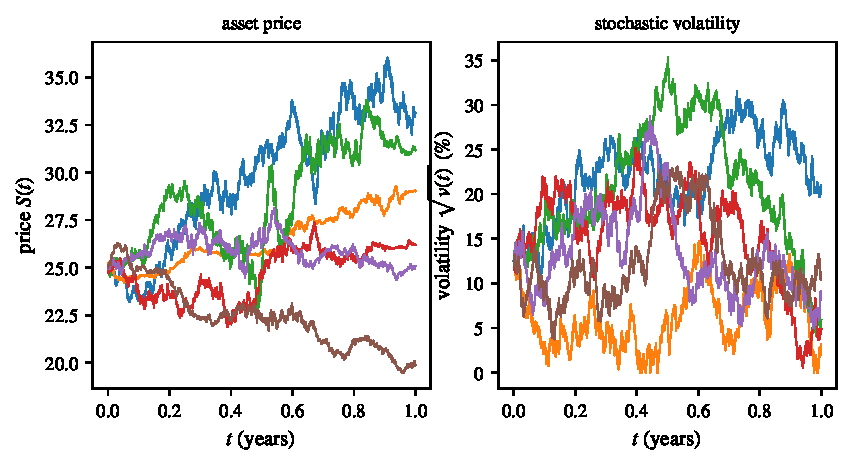
\includegraphics[width=0.95\textwidth]{images/heston_sim.pdf}
\caption{Monte Carlo simulation of the Heston model (six sample paths, full-truncation Euler scheme): the asset price $S(t)$ (left) and its stochastic volatility $\sqrt{v(t)}$ (right), with negative price--volatility correlation $\rho=-0.125$ to account for the leverage effect. Simulations of this kind are routinely used in finance for the pricing of plain vanilla and exotic options under stochastic volatility. Generated by \texttt{images/code\_for\_images/heston\_sim.py}.}
\label{fig:heston-sim}
\end{figure}

In Black--Scholes only the price $S(t)$ moves, and one protects oneself by holding stock.
In Heston one still hedges $dW_1$ by buying $S$, but for $dW_2$ there is nothing to buy: volatility is not exchanged.
One therefore needs another instrument, sensitive to volatility \emph{and} tradable --- another option.

\subsection{Hedging with two options}

Consider then two options $O_1$ and $O_2$ on the same stock, with maturities $T_1$ and $T_2$: $O_2$ is the \emph{target} option, the one the writer has sold, and $O_1$ is the instrument used to cover $dW_2$, with
\begin{equation}
T_1 > T_2 \ge t
\end{equation}
(the hedging option must outlive the target).
% CLAUDE NOTE: the notes write T₁ > T₂ > t; corrected to T₁ > T₂ ≥ t at the author's
% request (2026-07-06).
The writer's wealth is a portfolio of cash, a fraction $\Delta$ of stock (which takes care of $dW_1$), and a fraction $\Delta_1$ of the hedging option (which takes care of $dW_2$),
\begin{equation}
W(S,v,t) = \Pi(S,v,t) + \underbrace{\Delta(S,v,t)\, S}_{dW_1} + \underbrace{\Delta_1(S,v,t)\, O_1(S,v,t)}_{dW_2}
= O_2(S,v,t), \qquad \Delta, \Delta_1 \in \mathbb{R},
\end{equation}
where the last equality is replication: the portfolio must reproduce the sold option.
Therefore
\begin{equation}
\Pi(S,v,t) = O_2 - \Delta\, S - \Delta_1\, O_1
\quad\Longrightarrow\quad
d\Pi = dO_2 - \Delta\, dS - \Delta_1\, dO_1.
\end{equation}

To expand $dO_1$ and $dO_2$ we need the \emph{two-dimensional It\^o formula}, the natural extension of~\eqref{eq:ito-formula}: for $f[X(t), Y(t), t]$ with $dX = a\, dt + b\, dW_1$ and $dY = c\, dt + d\, dW_2$,
\begin{equation}
df = \biggl(\frac{\partial f}{\partial t} + a\frac{\partial f}{\partial x} + c\frac{\partial f}{\partial y} + \frac{1}{2}b^2\frac{\partial^2 f}{\partial x^2} + \frac{1}{2}d^2\frac{\partial^2 f}{\partial y^2} + \rho\, b\, d\,\frac{\partial^2 f}{\partial x\,\partial y}\biggr)dt + b\frac{\partial f}{\partial x}\, dW_1 + d\frac{\partial f}{\partial y}\, dW_2,
\end{equation}
the only novelty being the mixed term, generated by $dW_1\,dW_2 = \rho\,dt$.
Applied to the two option prices, and collecting the second-order operators into
\begin{equation}
\mathcal{D} = \frac{1}{2}v\, S^2\frac{\partial^2}{\partial S^2} + \frac{1}{2}\sigma^2 v\frac{\partial^2}{\partial v^2} + \rho\,\sigma\, v\, S\frac{\partial^2}{\partial S\,\partial v},
\end{equation}
this gives, for $i=1,2$,
\begin{equation}
dO_i = \biggl\{\frac{\partial O_i}{\partial t} + \mu S\frac{\partial O_i}{\partial S} + \kappa(\theta - v)\frac{\partial O_i}{\partial v} + \mathcal{D}\, O_i\biggr\}dt
+ \sqrt{v}\, S\,\frac{\partial O_i}{\partial S}\, dW_1
+ \sigma\sqrt{v}\,\frac{\partial O_i}{\partial v}\, dW_2.
\end{equation}

Now rearrange the portfolio differential as $d\Pi + \Delta\, dS + \Delta_1\, dO_1 = dO_2$ and compare the noise terms on the two sides.
Collecting $dW_1$ on the left gives $\sqrt{v}\,S\bigl(\Delta + \Delta_1\,\partial_S O_1\bigr)\,dW_1$, while the right carries $\sqrt{v}\,S\,\partial_S O_2\, dW_1$; collecting $dW_2$ gives $\Delta_1\,\sigma\sqrt{v}\,\partial_v O_1\, dW_2$ against $\sigma\sqrt{v}\,\partial_v O_2\, dW_2$.
The noise $dW_2$ cancels between the two members if
\begin{equation}
\sigma\sqrt{v}\,\frac{\partial O_2}{\partial v} = \Delta_1\,\sigma\sqrt{v}\,\frac{\partial O_1}{\partial v}
\quad\Longrightarrow\quad
\Delta_1 = \frac{\partial O_2/\partial v}{\partial O_1/\partial v}
\qquad \text{(the \emph{vega ratio})},
\end{equation}
the optimal option fraction: the two options are held in proportion to their volatility sensitivities, and the volatility noise is gone.
Likewise for $dW_1$,
\begin{equation}
\sqrt{v}\, S\,\frac{\partial O_2}{\partial S} = \sqrt{v}\, S\biggl(\Delta + \Delta_1\frac{\partial O_1}{\partial S}\biggr)
\quad\Longrightarrow\quad
\Delta = \frac{\partial O_2}{\partial S} - \Delta_1\frac{\partial O_1}{\partial S},
\end{equation}
the optimal stock fraction: the familiar delta hedge, with a \emph{correction} for the delta carried along by the hedging option.

\subsection{The Heston PDE}

With both noises cancelled, $d\Pi$ is now riskless, and by the no-arbitrage principle it must earn the risk-free rate,
\begin{equation}
d\Pi = r\,\Pi\, dt = r\,\bigl\{O_2 - \Delta\, S - \Delta_1\, O_1\bigr\}\,dt,
\end{equation}
with the optimal $\Delta$ and $\Delta_1$ substituted in.
On the other hand, $d\Pi$ can be computed from the It\^o expansions of $dO_1$ and $dO_2$ above; when the two expressions are equated, every term proportional to $\mu S$ cancels identically between the $O_2$ terms, the stock term, and the $O_1$ terms --- the same disappearance of the historical drift that blessed the Black--Scholes derivation.
% CLAUDE NOTE: these cancellations are exactly what the strikethrough marks in the
% handwritten notes (PDF 6, page 6) indicate.
What survives can be separated so that everything referring to $O_1$ stands on one side and everything referring to $O_2$ on the other:
\begin{equation}\begin{split}
&\biggl\{\frac{\partial O_1}{\partial t} + rS\frac{\partial O_1}{\partial S} + \kappa(\theta - v)\frac{\partial O_1}{\partial v} + \mathcal{D} O_1 - r O_1\biggr\}\biggl(\frac{\partial O_1}{\partial v}\biggr)^{\!-1}\\
&\qquad= \biggl\{\frac{\partial O_2}{\partial t} + rS\frac{\partial O_2}{\partial S} + \kappa(\theta - v)\frac{\partial O_2}{\partial v} + \mathcal{D} O_2 - r O_2\biggr\}\biggl(\frac{\partial O_2}{\partial v}\biggr)^{\!-1},
\end{split}\end{equation}
that is,
\begin{equation}
\frac{\mathrm{drift}(O_1) - r O_1}{\mathrm{vega}(O_1)} = \frac{\mathrm{drift}(O_2) - r O_2}{\mathrm{vega}(O_2)} = \lambda(S,v,t),
\end{equation}
a \emph{universal} function, the same for every option on this stock whatever its maturity --- the same separation-of-variables manoeuvre that produced the Vasi\v{c}ek identity in Chapter~6.
The function $\lambda$ is the \emph{price of volatility risk}: the extra return demanded per unit of volatility exposure, the exact analogue of the market price of risk $q$ of Chapter~6, and it appears here for the same reason as there --- because the risk source ($v$, like $r$) is not tradable.

Undoing the ratio, every option price must satisfy the \textbf{Heston PDE}:
\begin{equation}\label{eq:heston-pde}
\boxed{\ \underbrace{\frac{\partial O}{\partial t} + rS\frac{\partial O}{\partial S} + \frac{1}{2}vS^2\frac{\partial^2 O}{\partial S^2}}_{\text{Black--Scholes}} + \rho\,\sigma\, v\, S\frac{\partial^2 O}{\partial S\,\partial v} + \kappa(\theta - v)\frac{\partial O}{\partial v} + \frac{1}{2}\sigma^2 v\frac{\partial^2 O}{\partial v^2} - \lambda\frac{\partial O}{\partial v} = r\, O\ }
\end{equation}
The first three terms are exactly Black--Scholes; the new ones are the volatility drift and diffusion, the mixed derivative, and the $-\lambda\,\partial_v O$ term carrying the price of volatility risk (which may equivalently be folded into the drift as $[\kappa(\theta-v)-\lambda]\,\partial_v O$; in practice $\lambda$ is calibrated, or set to zero under the risk-neutral measure).
The equation duly collapses onto Black--Scholes when the volatility freezes ($\sigma=0$, $v=\text{const}$).

Is it solvable?
Remarkably, yes --- analytically, up to one integral.
For a European call the solution retains the Black--Scholes skeleton,
\begin{equation}
C(S,v,t) = S\,P_1 - X\,e^{-r(T-t)}\,P_2 \;\neq\; C_{\text{BS}},
\end{equation}
but the exercise probabilities $P_1$ and $P_2$ are no longer cumulative normals: they are computed numerically as the Fourier-type integrals
\begin{equation}
P_j = \frac{1}{2} + \frac{1}{\pi}\int_0^{\infty} \mathrm{Re}\bigl\{\cdots\bigr\}\, d\phi, \qquad j=1,2,
\end{equation}
whose integrands involve the model's characteristic function.\footnote{Heston's original insight was precisely that, although the PDF of the model is unknown, its \emph{characteristic function} is known in closed form; $P_1$ and $P_2$ then follow by inverse Fourier transform, evaluated by quadrature. This ``transform pricing'' technique has become a small industry of its own.}
The model earns its keep on the data as well: Dr\u{a}gulescu and Yakovenko showed that the Heston return distribution fits the Dow Jones index across time lags from one day to a year, reproducing the fat-tailed short-horizon distributions and their slow re-Gaussianization in one stroke\cite{DragulescuYakovenko2002}.
% CLAUDE NOTE: the Dragulescu-Yakovenko fit is from the course slides
% (Econophysics of the Financial Market Dynamics), added 2026-07-06.

The lesson of the chapter in one line: the market's deviations from Black--Scholes are systematic and measurable, and the models that capture them --- stable laws for the tails, stochastic volatility for the clustering --- remain tractable enough to price with.

\section{Summary: the stylized facts}
% CLAUDE NOTE: summary after the course slides and Cont's review (ReviewCont.pdf in
% "slides and other/"), added 2026-07-06.

It is useful to close the chapter by collecting the empirical regularities met along the way --- the \emph{stylized facts} of financial returns, so called because they hold, with remarkable universality, across markets, epochs, and asset classes\cite{Cont2001}.
\begin{enumerate}
    \item The geometric Brownian motion with constant volatility is not a realistic description of asset price dynamics.
    \item In liquid markets the returns are \emph{uncorrelated} random variables (the sign of efficient-market behaviour), but they are \emph{not independent}: higher-order correlations survive through the volatility.
    \item In the high-frequency limit the distribution of returns is leptokurtic and non-Gaussian, with heavy tails $P(r) \propto r^{-4}$ (the inverse quartic law), and it converges only slowly to a Gaussian over long horizons (\emph{aggregational Gaussianity}).
    \item The volatility is itself a stochastic process, with intermittent fluctuations (volatility clustering), long-range power-law autocorrelation, and a fat-tailed distribution (log-normal or inverse Gamma).
    \item Stochastic volatility models --- Stein--Stein, Heston, exponential OU --- provide a realistic description of these facts, give rise dynamically to non-Gaussian return distributions, and remain tractable enough for pricing, volatility forecasting, and simulation.
\end{enumerate}
One last application of the Fokker--Planck machinery awaits, and it takes us out of the market altogether: the distribution of wealth in a society.
